%
% Master thesis template for Ghent University (2021)
%
%
%  !!!!!!!!!!!!!!!!!!!!!!!!!!!!!!!!!!!!!!!!!!!!!!!!!!!!!!!!!!!!
%  !!  MAKE SURE TO SET lualatex OR xelatex AS LATEX ENGINE  !!
%  !!!!!!!!!!!!!!!!!!!!!!!!!!!!!!!!!!!!!!!!!!!!!!!!!!!!!!!!!!!!
%  !! For overleaf:                                          !!
%  !!     1. click gear icon in top right                    !!
%  !!     2. select `lualatex` in "latex engine"             !!
%  !!     3. click "save project settings"                   !!
%  !!                                                        !!
%  !!!!!!!!!!!!!!!!!!!!!!!!!!!!!!!!!!!!!!!!!!!!!!!!!!!!!!!!!!!!
%
%
%  History
%    2014         Doctoral Thesis of Bruno Volckaert
%    2017         Adapted to master thesis by Jerico Moeyersons
%    2018         Cleanup by Merlijn Sebrechts
%    2021         Update by Marleen Denert and Merlijn Sebrechts with feedback from Leen Pollefliet
%
%  Latest version
%    https://github.com/galgalesh/masterproef-template
%
\documentclass[11pt,a4paper,openany]{book}
\usepackage[a4paper,includeheadfoot,margin=2.50cm]{geometry}

\setlength{\parindent}{0cm}           % indent of the first sentence of a paragraph
\setlength{\parskip}{1em}             % space between paragraphs

\renewcommand{\baselinestretch}{1.2}  % stretch horizontal space between everything

\usepackage[hyphens]{url} % Break line on hyphens in long urls
\usepackage{graphicx}
\graphicspath{{images/}}
\usepackage{pdfpages}
\usepackage{enumitem}
\usepackage{float}
\usepackage{caption}
\usepackage{subcaption}
\usepackage[toc,page]{appendix}
\usepackage{fontspec}
\usepackage[T1]{fontenc}

% Don't indent table of contents, list of figures, and list of tables
\usepackage{tocloft}
\setlength{\cftsecindent}{0pt}    % Remove indent for \section
\setlength{\cftsubsecindent}{0pt} % Remove indent for \subsection
\setlength{\cftfigindent}{0pt}    % remove indentation from figures in lof
\setlength{\cfttabindent}{0pt}    % remove indentation from tables in lot

% To generate fake lorem ipsum text
\usepackage{lipsum}


%
% UGent style guide
%
\setmainfont[
	Path=fonts/,
	BoldFont      =UGentPannoText-SemiBold.ttf,
	ItalicFont    =UGentPannoText-Normal.ttf,
	ItalicFeatures={FakeSlant=0.3},
	BoldItalicFont=UGentPannoText-SemiBold.ttf,
    BoldItalicFeatures={FakeSlant=0.3},
]{UGentPannoText-Normal.ttf}
\urlstyle{same} % Also use the default font for URLs


% If you want left justified text, uncomment the line below. Note: left justified text is probably not easier to read: https://graphicdesign.stackexchange.com/a/154231/169301
%\usepackage[document]{ragged2e} % Left justify all text




% Style Chapter titles so they have the chapter number in grey.
\usepackage{color}
\definecolor{chaptergrey}{rgb}{0.5,0.5,0.5}
\usepackage[explicit, pagestyles]{titlesec}
\titleformat{\chapter}[display]{\bfseries}{\color{chaptergrey}\fontfamily{pbk}\fontsize{80pt}{100pt}\selectfont\thechapter}{0pt}{\Huge #1}
\titlespacing*{\chapter}{0pt}{-80pt}{30pt}


% Header showing chapter number and title and footer showing page number
\newpagestyle{fancy}{%
  \sethead{} % left
          {} % center
          {\Large\thechapter~~\chaptertitle} %right
  \setfoot{} % left
          {\thepage} % center
          {} %right
  \setheadrule{0pt}
}
\pagestyle{fancy}

% Header showing chapter title and footer showing page number
\newpagestyle{numberless}{%
  \sethead{} % left
          {} % center
          {\Large\chaptertitle} %right
  \setfoot{} % left
          {\thepage} % center
          {} %right
  \setheadrule{0pt}
}

\usepackage{minted}                                    % for modern code highlighting
\newenvironment{code}{\captionsetup{type=listing}}{}   % To get multiline code fragments working: https://tex.stackexchange.com/a/53540/72273

\PassOptionsToPackage{hyphens}{url}
\usepackage{hyperref}
\usepackage{url}

\usepackage[numbers]{natbib}       % For bibliography; use numeric citations
\bibliographystyle{IEEEtran}
\usepackage[nottoc]{tocbibind}     % Put Bibliography in ToC

%
% Defines \checkmark to draw a checkmark
%
\usepackage{tikz}
\def\checkmark{\tikz\fill[scale=0.4](0,.35) -- (.25,0) -- (1,.7) -- (.25,.15) -- cycle;}

%
% For tables
%
\usepackage{booktabs}
\usepackage{array}
\usepackage{ragged2e}  % for '\RaggedRight' macro (allows hyphenation)
\newcolumntype{L}[1]{>{\raggedright\let\newline\\\arraybackslash\hspace{0pt}}m{#1}}
\newcolumntype{C}[1]{>{\centering\let\newline\\\arraybackslash\hspace{0pt}}m{#1}}
\newcolumntype{R}[1]{>{\raggedleft\let\newline\\\arraybackslash\hspace{0pt}}m{#1}}

%
% Support for splitting Dutch words correctly
%
\usepackage{polyglossia}
\setdefaultlanguage[babelshorthands=true]{dutch}

% Manually specify additional hypnations for words
%
% Translated strings. If these aren't set, the English words are used.
%
\addto\captionsenglish{%
  \renewcommand{\contentsname}%
    {Inhoudsopgave}%
}


\renewcommand\appendixtocname{Bijlagen}
\renewcommand\appendixpagename{Bijlagen}
\renewcommand{\listoflistingscaption}{Lijst van listings}

%
% Set the title and your name
%
\title{de titel}
\author{de auteur}

%
%  END OF HEADER
%  The actual latex document content starts here.
%
\begin{document}
%download het voorblad van plato
\frontmatter
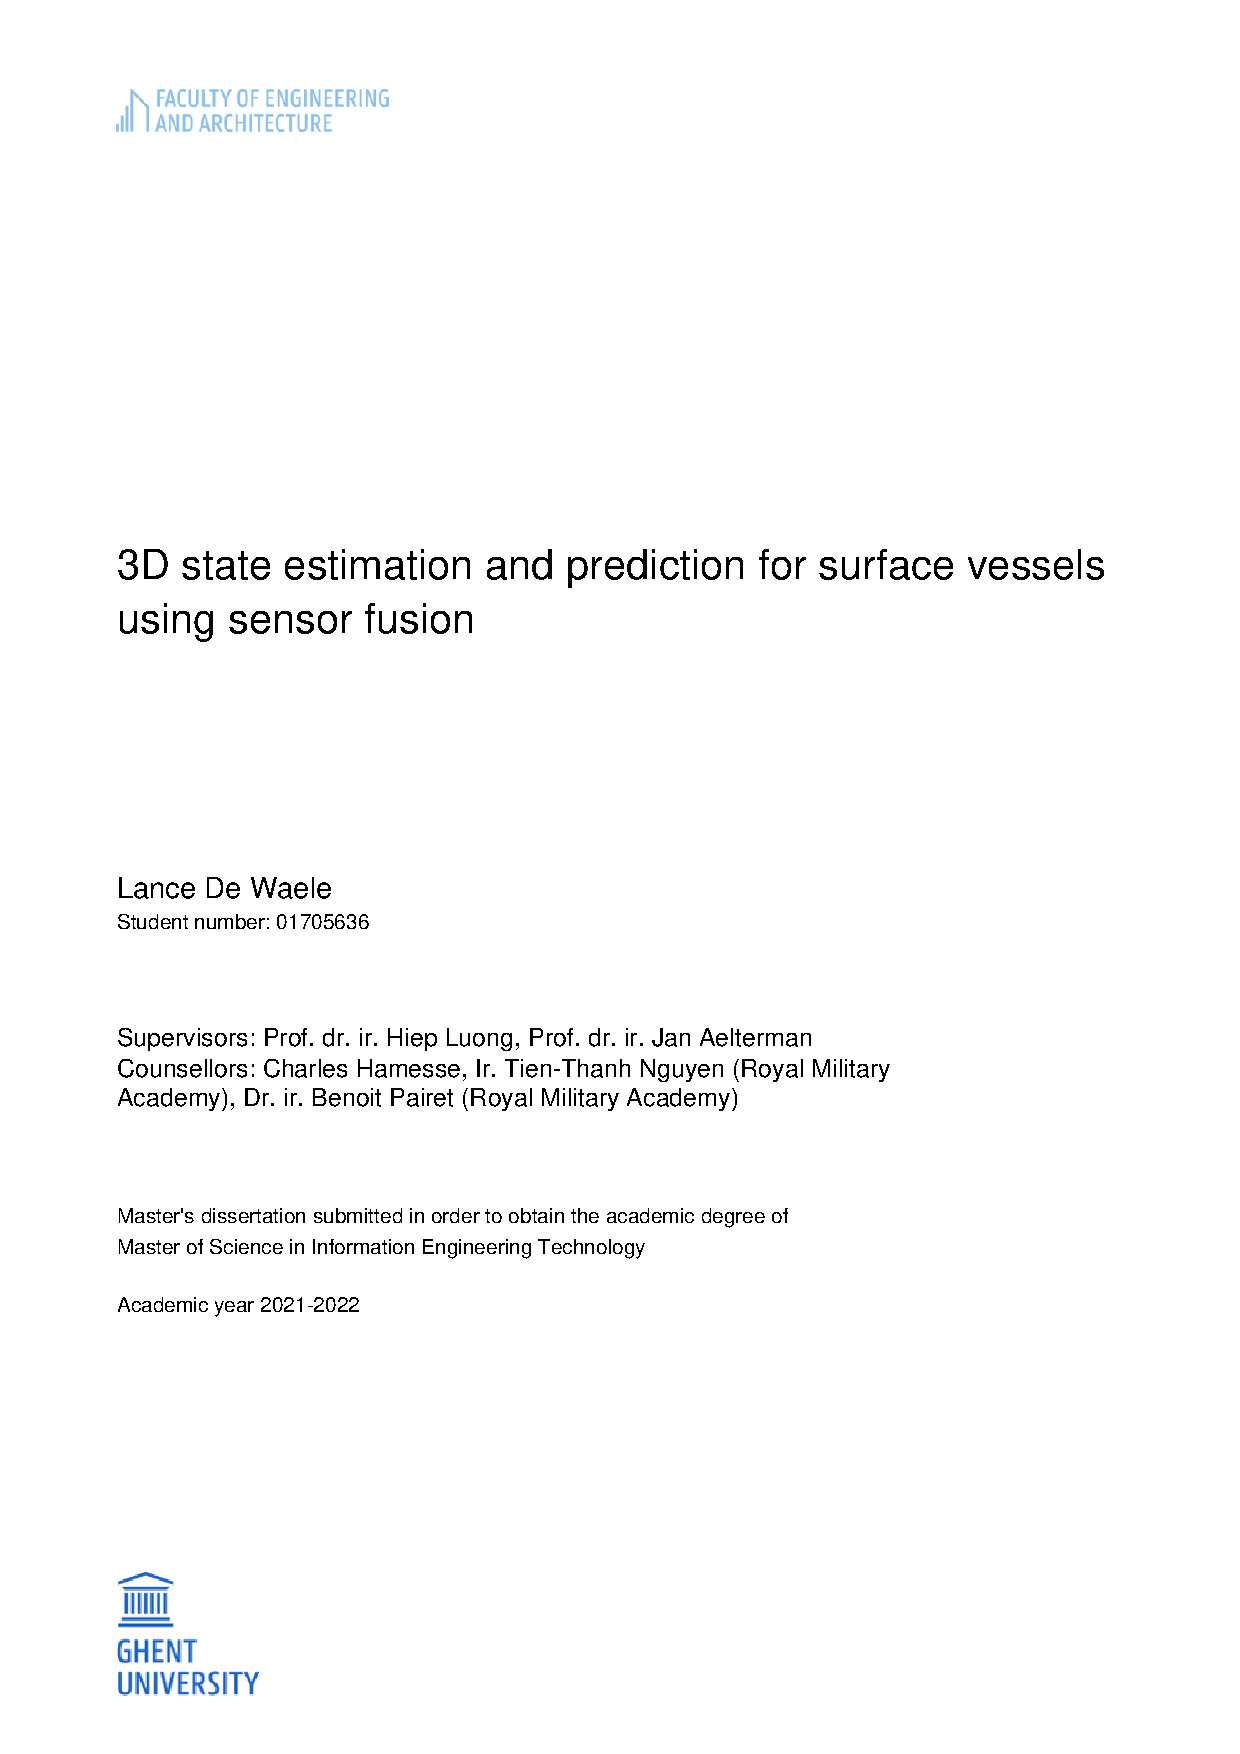
\includepdf{voorblad.pdf}

% White page
\newpage\thispagestyle{empty}\mbox{}
\mainmatter
% Word of thanks
\chapter*{Dankwoord}

\textit{Vul aan.}

\lipsum[2-4]


% White page
\newpage\thispagestyle{empty}\mbox{}

% Om het extended abstract te schrijven kan je de IEEE conference proceedings template gebruiken. Die staat ook op Overleaf: https://www.overleaf.com/latex/templates/ieee-conference-template/grfzhhncsfqn. Voeg dit toe als .pdf
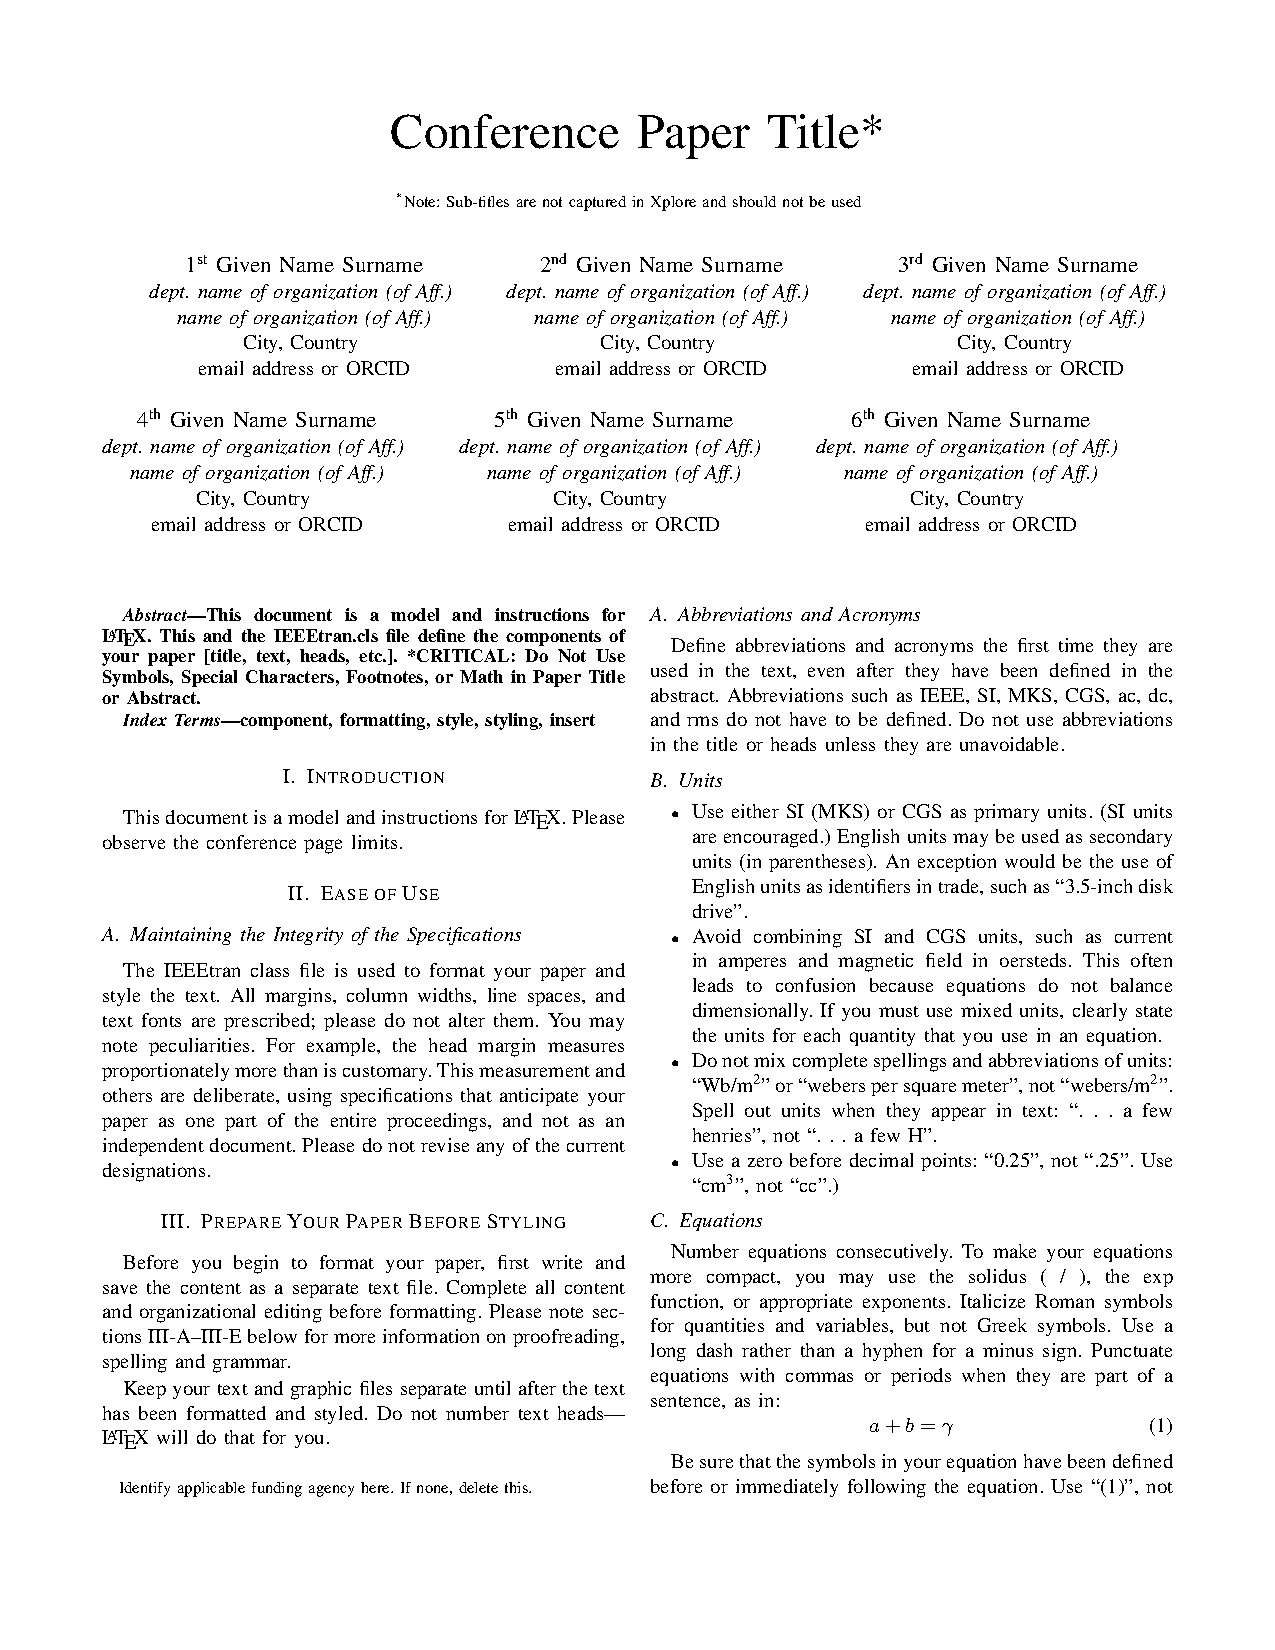
\includepdf[pages={-}]{abstract.pdf}  % Extended Abstract
\tableofcontents                      % Table of Contents
\newpage
\listoffigures                        % List of figures
\newpage
\listoftables                         % List of tables
\newpage
\listoflistings                       % List of listings (code fragments)

%
% Include the main chapters of the thesis below
%

\chapter*{Inleiding}
\chaptermark{Inleiding}
\addcontentsline{toc}{chapter}{Inleiding}  
\label{chap:intro}

Vul aan.

\lipsum[66-68]
\lipsum[66-68]
\lipsum[66-68]
\lipsum[66-68]

\chapter{Titel van het eerste hoofdstuk}
\label{chap:rel_work}

\lipsum[2-4]

\section{Sectie titel}
\label{sec:related_work}

\lipsum[3-4]

\begin{table}[tbp]
	\centering
	\captionsetup{justification=centering}
	\caption[Overzicht resource-allocatieschema's]{Overzicht resource-allocatieschema's \\
		A=Algoritme, P=Protocol, F=Framework S=Simulator, C=Cloud, ILP=Integer Linair Programming, GH = Greedy Heuristic, SBP=Stochastic Bin Packing, MINLP=Particle swarm, RR=Round-Robin, SA=Simulated Annealing, SMT=Satisfiabilty Module Theory, FFD=First Fit Decreasing, MI(N)=Mixed Integer (Non-), SPLE=Software Product Line Engineering, L=Lijst, G=Graaf, B=Boom, FN=Fysieke node, Mig=Migraties, (?)=Niet vermeld}
	\label{tab:resallocschemes}
	\resizebox{\textwidth}{!}{%
	\begin{tabular}{L{4cm} l C{2cm} c c c c}
		\toprule
		Naam & Jaar & Type  & A | F | P  & Invoer & Uitvoer & Getest  \\ \midrule
		Alicherry et al.~\cite{Alicherry2012} & 2012 & k-sneden & A & G & par\{G\} & S \\
		MCRVMP~\cite{Biran2012} & 2012 & ILP \& GH & A & B\{netwerk\} & VM-plaatsing & C\\
		\bottomrule
	\end{tabular}}
\end{table}

\lipsum[3-4]

In Tabel~\ref{tab:resallocschemes} wordt een overzicht weergegeven ...



\chapter{Titel tweede hoofdstuk}
\label{chap:evaluation}

Vul aan.

\lipsum[9-10]

\section{Sectie titel}
\label{sec:scalable_faafo}

Vul aan.

\lipsum[10-12]
Voorbeeld figuur.

\begin{figure}
	\centering
	\subcaptionbox{Uitvoer van Rally \label{fig:evaluation_rally1}}{%
		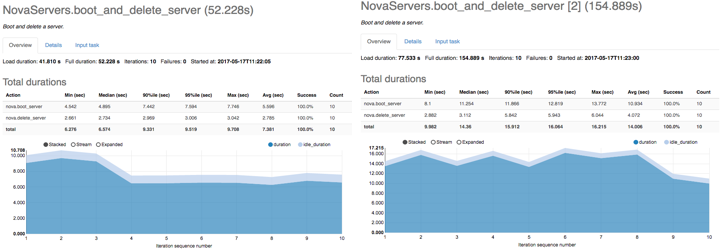
\includegraphics[width=1.00\textwidth]{Dia3}%
	}\par\medskip
	\subcaptionbox{Uitvoer van de monitorapplicatie \label{fig:evaluation_rally2}}{%
		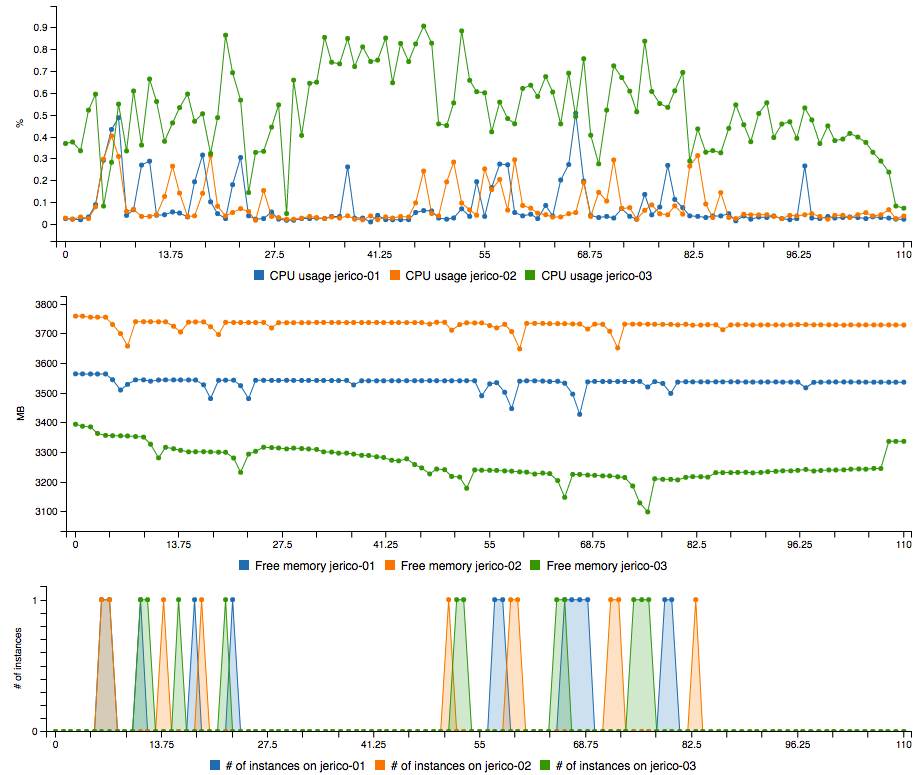
\includegraphics[width=1.00\textwidth]{rally_evaluation}%
	}
	\caption{Evaluatie met Rally - Resultaten}
	\label{fig:evaluation_rally}
\end{figure}

\chapter{Titel derde hoofdstuk}

Vul aan.


\lipsum[20-24]

\section{Sectie titel}

Vul aan.

\lipsum[32-34]
\section{Sectie titel2}

\lipsum[6-8]

Voorbeeld figuur.

\begin{figure}
	\centering
	\begin{subfigure}{\textwidth}
		\centering
		\centerline{
			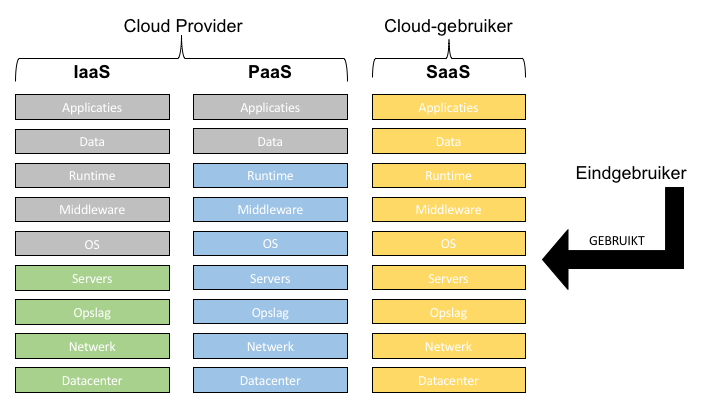
\includegraphics[scale=0.47]{cloud_rollen}
		}
	\end{subfigure}
	\caption{Cloudstakeholders met de bijhorende cloudvorm.}
	\label{fig:cloud_rollen}
\end{figure}

\subsection*{Subtitel}
\addcontentsline{toc}{subsection}{Subtitel}  
Vul aan
\subsection{Functie is\_isbn}

Voorbeeld listing.

\begin{code}
\inputminted{python}{isbn.py}
\caption{Functie is\_isbn}
\end{code}

\pagestyle{numberless} 
\chapter*{Conclusie}
\chaptermark{Conclusie}
\addcontentsline{toc}{chapter}{Conclusie}  


Vul aan.


\lipsum[2-4]

\phantomsection
\section*{Ethische en maatschappelijke reflectie}
\addcontentsline{toc}{section}{Ethische en maatschappelijke reflectie}  

Vul aan.

Meer informatie kan je opzoeken op https://www.sdgs.be/nl/sdgs


\lipsum[2-4]

\renewcommand\bibname{Referenties}
\bibliography{referenties}

\pagestyle{empty}
\begin{appendices}
\section*{Bijlage 1}
\addcontentsline{toc}{section}{Bijlage 1}  

Toelichting bijlage.

\lipsum[6-8]

\newpage
\section*{Bijlage 2}
\addcontentsline{toc}{section}{Bijlage 2}  

Toelichting bijlage.

\lipsum[16-28]

\end{appendices}

\end{document}
